\documentclass[a4paper]{article}
\usepackage[pdftex]{graphicx}
\usepackage[utf8]{inputenc}
\usepackage{enumerate}
\usepackage{icomma}
\usepackage{siunitx}
\sisetup{locale=DE}
\usepackage{amssymb}
\usepackage{tikz}
\usepackage{href-ul}
\hypersetup{
	colorlinks=true,
	linkcolor=blue,
	urlcolor=blue}
\usepackage{geometry}
\geometry{a4paper, top=15mm, left=15mm, right=15mm, bottom=15mm,
	headsep=10mm, footskip=12mm}

\begin{document}
	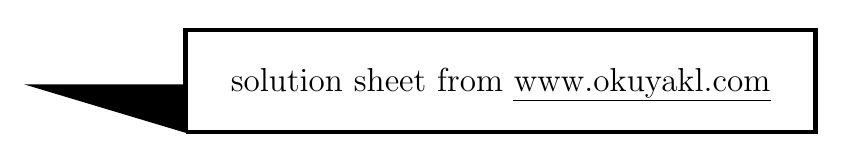
\begin{tikzpicture}(10,3)
		\draw[ultra thick](2,0) --(10,0) -- (10,1.3) --(2,1.3) -- (2,0);
		\draw[fill=black](2,0)-- (0,.6) -- (2,.6) -- (2,0);
		\node at (6,.6) {\large solution sheet from \href{http://www.okuyakl.com}{www.okuyakl.com}};
	\end{tikzpicture}
	\vspace{0.5 cm}
	
	SOLUTION
	
	\noindent{\bf Task 1.}\\
	We first calculate the volume of such a ball:
	$$V={4\over 3}\pi r^3 = {4\over 3}\pi \cdot(\SI{1}{\meter})^3 =\SI{4,19}{\meter }^3$$
	$1000~dm^3 = \SI{1}{\meter}^3 \quad \Rightarrow \quad \SI{1}{\meter}^3$ weighs $\SI{30}{\kilogram} \quad \Rightarrow $ the ball weighs:
	$$m_K=\SI{4,19}{\meter}^3\cdot \SI{30}{\kilogram\per \meter^3}=\SI{126}{\kilogram}$$
	You can't carry this ball alone; it is too heavy (and too unwieldy).
	
	\noindent{\bf Task 2.}\\
	By rearranging the formula for the spherical volume, we get the radius:
	$$
	\renewcommand{\arraystretch}{2}
	\begin{array}{rcll}
		V &=& {4 \over 3} \pi r^3 & | \cdot {3 \over 4 \pi}\\
		{3 V\over 4 \pi}&=& r^3 &|\sqrt[3]{\quad}\\
		\sqrt[3]{3 V\over 4 \pi}&=& r &={d\over 2}\\
		d&=& 2\cdot \sqrt[3]{3 V\over 4 \pi} &(*)
	\end{array}
	$$
	\noindent{\bf task 2.a)}\\
	We substitute $V=\SI{1}{\meter}^3$ into $(*)$:
	$$d= 2\cdot \sqrt[3]{3\cdot \SI{1}{\meter}^3 \over 4 \pi}= \SI{1,24}{\meter}$$
	
	\noindent{\bf Task 2.b)}\\
	We substitute $V=\SI{49}{\centi\meter}^3$ into $(*)$:
	$$d= 2\cdot \sqrt[3]{3\cdot \SI{49}{\centi\meter}^3 \over 4 \pi}= \SI{4,54}{\centi\meter}$$
	
	\noindent{\bf Task 3.}\\
	The can has a height of $h=6r$. The cylinder volume is therefore:
	$$ V_Z = \pi r^2 \cdot h= 6\pi r^3$$
	The volume of the three balls is:
	$$V_{3B} = 3\cdot {4 \over 3} \pi r^3 = 4 \pi r^3 $$
	The volume of the spaces is the difference between them; the percentage of the cylinder volume is calculated using the formula:
	$$p\% = \left({V_{Z}-V_{3B} \over V_{Z}}\right)\cdot 100\% = \left(1-{V_{3B} \over V_{Z }}\right)\cdot 100\% = \left(1- {4\pi r^3 \over 6 \pi r^3}\right)\cdot 100\% = \left(1-{4\over 6}\right)\cdot 100\% = 33\%$$
	
	\noindent{\bf Task 4.}\\
	We take the spherical volume as a reference and equate the cylinder and cone volumes one after the other and solve for the respective height $h$.\\
	Height of the cylinder:
	$$
	\renewcommand{\arraystretch}{2}
	\begin{array}{rcll}
		V_K &=& V_Z \\
		{4 \over 3} \pi r^3 &=& \pi r^2 \cdot h_Z &|: \pi r^2\\
		{4 \over 3} r &=& h_Z\\
	\end{array}
	$$
	Height of the cone:
	$$
	\renewcommand{\arraystretch}{2}
	\begin{array}{rcll}
		V_K &=& V_{Ke} \\
		{4 \over 3} \pi r^3 &=& {1\over 3} \pi r^2 \cdot h_{Ke} &|: {1\over 3} \pi r^2\\
		4 r &=& h_{Ke}\\
	\end{array}
	$$
	If you compare the height of these three bodies, the cylinder is the lowest, the sphere with height $2r$ is second, and the cone is the highest.
	
	\noindent{\bf Task 5.}\\
	The volume of a drop is:
	$$V_T={4 \over 3} \pi (\SI{2}{\milli\meter})^3 =\SI{33.5}{\milli\meter}^3$$
	The number of drops in a week is 30 drops per minute:
	$$n=7\cdot 24 \cdot 60 \cdot 30 = 302400$$
	The amount of water that is lost is calculated as the number of drops times the drop volume:
	$$V = n \cdot V_T = 302400 \cdot \SI{33.5}{\milli\meter}^3 \approx \SI{1e7}{\milli\meter}^3 = \SI{10}{\ deci\meter}^3 = 10~l$$
	
	\noindent{\bf Task 6.}\\
	The radius $r$ increases by a tenth and is then $1.1~r$. The percentage increase in volume is then calculated using the formula:
	$$\left({V_{new} \over V_{old}}-1\right) \cdot 100\% = \left({{4\over 3} \pi (1,1r)^3 \over { 4\over 3} \pi r^3}-1 \right)\cdot 100\% =
	\left({1,1^3 \over 1}-1\right)\cdot 100\% = (1.331-1)\cdot 100\% = 33\%$$
	
	\noindent{\bf Task 7.}\\
	Let the radius of the sphere be $r$ and its volume $V_K$. The edge length of the cube is then $2r$, the cube volume is $V_W=(2r)^3=8r^3$.
	The percentage of the volume of the inscribed sphere is therefore:
	$${V_K \over V_W}\cdot 100\% = {{4 \over 3} \pi r^3 \over 8 r^3}= {{4 \over 3} \pi \over 8} \cdot 100 \% = 52\%$$
	
	\noindent{\bf Task 8. a)}\\
	The total surface area of the earth is:
	$$ O_E= 4\pi r^2 = 4 \pi \cdot (\SI{6370}{\kilo\meter})^2=\SI{5,1e8}{\kilo\meter}^2$$
	The water would be evenly distributed over this area; The water depth $h_E$ would be:
	$$V = O_E \cdot h_E \quad \Rightarrow \quad h_E = {V\over O_E} = {\SI{1,4e9}{\kilo\meter}^3 \over \SI{5,1e8}{\ kilo\meter}^2 }= \SI{2.7}{\kilo\meter} $$
	
\noindent{\bf Exercise 8. b)}\\
The surface area of the moon Europa is:
$$O_M= 4\pi r^2 = 4 \pi \cdot (\SI{1560}{\kilo\meter})^2=\SI{3,1e7}{\kilo\meter}^2$$
The average water depth $h_M$ is:
$$V = O_E \cdot h_M \quad \Rightarrow \quad h_M = {V\over O_M} = {2 \cdot \SI{1.4e9}{\kilo\meter}^3 \over \SI{3.1e7 }{\kilo\meter}^2 }= \SI{90}{\kilo\meter} $$

\noindent{\bf Task 9. a)}\\
The volume of both spheres with radius $1.5a$ is equal to the volume of the combined sphere with the new radius $R$. We equate both volumes and solve for the new radius:
$$
\renewcommand{\arraystretch}{2}
\begin{array}{rcll}
	2\cdot {4 \over 3} \pi (1,5~a)^3 &=& {4\over 3} \pi R^3 &|: {4\over 3} \pi \\
	2\cdot (1.5~a)^3 &=& R^3 &|\sqrt[3]{\quad}\\
	\sqrt[3]{2}\cdot 1.5~a&=& R\\
	R&=& 1.89~a
\end{array}
$$

\noindent{\bf Task 9. b)}\\
The surface of the two spheres is:
$$O_{2K} = 2\cdot 4\pi \cdot (1.5~a)^2 = 56.5~a^2$$
The new surface of the merged sphere is:
$$O_{new} = 4\pi \cdot (1.89~a)^2 = 44.9~a^2$$
We get the percentage of the new surface compared to the old one with:
$$ {O_{new} \over O_{2K}} \cdot 100\% = 79.4\%$$

\noindent{\bf Task 10.}\\
The radius of the orange without peel is
$$r = {\SI{8.0}{\centi\meter}\over 2} -\SI{0.6}{\centi\meter} = \SI{3.4}{\centi\meter} $$ The volume of the pulp is therefore:
$$V= {4 \over 3} \pi \cdot (\SI{3,4}{\centi \meter})^3 = \SI{165}{\centi \meter}^3 = \SI{165 }{\milli\liter}$$
The juice content of this is 70%; multiplied by 5 oranges this gives a juice amount of:
$$V_{ges}=\SI{165}{\milli\liter}\cdot 0.7 \cdot 5 =\SI{576}{\milli\liter}$$

\noindent{\bf Task 11. a)}\\
The following applies: $$r={\SI{4.27}{\centi\meter} \over 2}=\SI{2.135}{\centi\meter} $$
This gives us for the surface:
$$O= 4\cdot \pi r^2= \SI{57.28}{\centi\meter}^2$$
And for the volume:
$$V={4\over 3} \pi r^3=\SI{40.76}{\centi \meter}^3$$
\noindent{\bf Exercise 11. b)}\\
$$ \textnormal{density}\, \varrho = { \textnormal{mass}\,m \over \textnormal{volume} \, V }=
{\SI{45.9}{\gram} \over \SI{40.76}{\centi \meter}^3} = \SI{1.13 }{\gram \per \centi \meter^3} $$
The density of water is lower: $\varrho_{water}=\SI{1}{\gram \per \centi\meter^3} $.\\
\noindent{\bf Exercise 11. c)}\\
The golf ball sinks into the lake; he can not swim. [He could swim in the Dead Sea $\varrho=\SI{1,24}{\gram \per \centi\meter^3}$.]

\begin{center}
	\includegraphics[width=7 cm]{../../viecher/eendcomic.pdf}
	
	Here you can go back to the \href{https://www.okuyakl.de/math/m10kuvolL217/ae217.pdf}{task sheet}
\end{center}

\end{document}